
\documentclass [PhD] {uclathes}

\usepackage{graphicx}
\graphicspath{ {./figures/} }
\usepackage{cite}
\usepackage[colorlinks]{hyperref}
\hypersetup{
     colorlinks = true,
     linkcolor = blue,
     anchorcolor = blue,
     citecolor = blue,
     filecolor = blue,
     urlcolor = blue
}


% \input {mymacros}                         % personal LaTeX macros

%%%%%%%%%%%%%%%%%%%%%%%%%%%%%%%%%%%%%%%%%%%%%%%%%%%%%%%%%%%%%%%%%%%%%%
%
% Usually things live in separate flies.
%
% \input {prelim}                           % preliminary page info

%%%%%%%%%%%%%%%%%%%%%%%%%%%%%%%%%%%%%%%%%%%%%%%%%%%%%%%%%%%%%%%%%%%%%%%%
%                                                                      %
%                          PRELIMINARY PAGES                           %
%                                                                      %
%%%%%%%%%%%%%%%%%%%%%%%%%%%%%%%%%%%%%%%%%%%%%%%%%%%%%%%%%%%%%%%%%%%%%%%%

\title          {Discovering Data-Driven Actionable Intelligence\\
for Clinical Decision Support}
\author         {Ahmed M. Alaa H. H. Ibrahim}
\department     {Electrical and Computer Engineering}
% Note:  degreeyear should be optional, but as of  5-Feb-96
% it seems required or you get a year of ``2''.   -johnh
\degreeyear     {2019}

%%%%%%%%%%%%%%%%%%%%%%%%%%%%%%%%%%%%%%%%%%%%%%%%%%%%%%%%%%%%%%%%%%%%%%%%

\chair          {Mihaela van der Schaar}
\member         {Douglas Bell}
\member         {Patricia Ganz}
\member         {Yahya Rahmat-Samii}
\member         {Greg Pottie}



%%%%%%%%%%%%%%%%%%%%%%%%%%%%%%%%%%%%%%%%%%%%%%%%%%%%%%%%%%%%%%%%%%%%%%%%

\dedication     {\textsl{To my parents and my brothers.}}

%%%%%%%%%%%%%%%%%%%%%%%%%%%%%%%%%%%%%%%%%%%%%%%%%%%%%%%%%%%%%%%%%%%%%%%%

\acknowledgments {
I would not have been able to complete this dissertation without the help and support
of my family, my adviser, my colleagues and friends. I am deeply grateful.

First, I wish to thank my adviser, Professor Mihaela van der Schaar, for her kindness~and unyielding support. This dissertation would not have been possible without her~research~vision. Her new ideas, insights, opportunities and willingness to intrepidly explore multidisciplinary research terrains have had a profound impact on my development as a researcher. I am deeply grateful for her invaluable support and immense help. Thank you for everything, Mihaela. I also thank the other members of my dissertation committee, Professor Greg Pottie, Professor Yahya Rahmat-Samii, Professor Patricia Ganz, and Dr. Douglas Bell for their valuable perspectives and thoughtful feedback. 

I would also like to thank all of my co-authors and collaborators at UCLA; Jinsung Yoon, Scott Hu, William Zame, Changhee Lee, Kartik Ahuja, William Hsu, Kyeong Moon and Martin Cadeiras. It has been a great privilege to be able to work with such talented people. I have also been fortunate to enjoy the collegiality of my labmates; Onur Atan, Trent Kyono, William Whoiles, Yangbo Song, Simpson Zhang, Jie Xu and Yuanzhang Xiao, with whom I had many insightful research discussions. I would also like to thank my friends at UCLA for their companionship and support. I especially want to thank Ahmed Hareedy, Mohammed Karmoose, Yahya Ezzeldin, Omar Hussien, Moustafa Alzantot, and Safa Cicek. 

I have been so lucky to spend some time on the other side of the Atlantic as a visiting student at Oxford University. There, I was fortunate to work with my colleagues at Oxford University, Ioana Bica, James Jordon, Bryan Lim, and Michael Weisz, and my colleagues at Cambridge University, Yao Zhang, Zhaozhi Qian, Alexis Bellot, and Daniel Jarrett.     

During my visit in the UK, I was blessed to be able to collaborate with many clinicians who provided me with the clinical data, guidance and feedback that made the clinical application of my work come to life. I would like to especially thank Dr. Jem~Rashbass~(National~Director for Disease Registration at Public Health England) for granting me access to the UK breast cancer registry data, and Dr Janet Allen (Director of Strategic Innovation at the UK Cystic Fibrosis Trust) for enabling my access to the UK Cystic Fibrosis registry. I would also like to thank my clinical collaborators at Cambridge University, Andres Floto, Fiona Gilbert, Emanuele Di Angelantonio, James Rudd, and my collaborator at Queen Mary University of London, Deepti Gurdasani.  

Finally, and most importantly, I wish to thank my parents, Hadeel and Alaa, and my borthers, Ali and Sherif for their love and support. No words can express what your encouragement and support have meant to me. 
}

%%%%%%%%%%%%%%%%%%%%%%%%%%%%%%%%%%%%%%%%%%%%%%%%%%%%%%%%%%%%%%%%%%%%%%%%

\vitaitem   {2011}
                {Bachelor in Communications and Computer Engineering,\\ 
                Cairo University, Cairo, Egypt}
\vitaitem   {2011--2014}
                {Teaching Assistant, Communications Engineering Department,\\ Cairo University, Cairo, Egypt}
\vitaitem   {2014}
                {Master of Science in Electronics and Communications Engineering,\\
Cairo University, Cairo, Egypt}
\vitaitem   {2014}
                {Graduate Division Fellowship, Electrical Engineering,\\ University of California, Los Angeles.}
\vitaitem   {2014--2019}
                {Research Assistant,\\ University of California, Los Angeles.}
\vitaitem   {2017--2018}
                {Recognized PhD Student,\\ University of Oxford, United Kingdom.}

%%%%%%%%%%%%%%%%%%%%%%%%%%%%%%%%%%%%%%%%%%%%%%%%%%%%%%%%%%%%%%%%%%%%%%%%

\publication {\textbf{A. M. Alaa}, T. Bolton, E. Di Angelantonio, J. H. F. Rudd, M. van der Schaar, ``Cardiovascular Disease Risk Prediction using Automated Machine Learning: A Prospective Study of 423,604 UK Biobank Participants,'' \textit{PloS One}, 2019.

\vspace{-.15in}
\hspace{-.3in}
\textbf{A. M. Alaa}, M. van der Schaar, ``Demystifying Black-box Models with Symbolic Metamodels,'' \textit{Neural Information Processing Systems} (NeurIPS), 2019.

\vspace{-.15in}
\hspace{-.3in}
\textbf{A. M. Alaa}, M. van der Schaar, ``Attentive State-Space Modeling of Disease Progression,'' \textit{Neural Information Processing Systems} (NeurIPS), 2019.

\vspace{-.15in}
\hspace{-.3in}
\textbf{A. M. Alaa}, M. van der Schaar, ``Validating Causal Inference Models via Influence Functions,'' \textit{International Conference on Machine Learning} (ICML), 2019.

\vspace{-.15in}
\hspace{-.3in}
I. Bica, \textbf{A. M. Alaa}, M. van der Schaar, ``Estimating Counterfactual Treatment Outcomes over Time through Adversarially Balanced Representations,'' \textit{NeurIPS Machine Learning for Health Workshop}, 2019.

\vspace{-.15in}
\hspace{-.3in}
I. Bica, \textbf{A. M. Alaa}, M. van der Schaar, ``Time Series Deconfounder: Estimating Treatment Effects over Time in the Presence of Hidden Confounders,'' \textit{NeurIPS Machine Learning for Health Workshop}, 2019.

\vspace{-.15in}
\hspace{-.3in}
C. Lee, W. R. Zame, \textbf{A. M. Alaa}, M. van der Schaar, ``Temporal Quilting for Survival Analysis,'' \textit{International Conference on Artificial Intelligence and Statistics} (AISTATS), 2019.

\vspace{-.15in}
\hspace{-.3in}
\textbf{A. M. Alaa}, M. van der Schaar, ``Prognostication and Risk Factors for Cystic Fibrosis via Automated Machine Learning,'' \textit{Scientific Reports}, 2018.

\vspace{-.15in}
\hspace{-.3in}
\textbf{A. M. Alaa}, M. van der Schaar, ``Bayesian Nonparametric Causal Inference: Information Rates \& Learning Algorithms,'' \textit{IEEE Journal of Selected Topics in Signal Processing}, 2018.

\vspace{-.15in}
\hspace{-.3in}
J. Yoon, W. R. Zame, A. Banerjee, M. Cadeiras, \textbf{A. M. Alaa}, M. van der Schaar, ``Personalized survival predictions via Trees of Predictors: An application to cardiac transplantation,'' \textit{PloS One}, 2018.

\vspace{-.15in}
\hspace{-.3in}
B. Lim, \textbf{A. M. Alaa}, M. van der Schaar, ``Forecasting Treatment Responses Over Time Using Recurrent Marginal Structural Networks,'' \textit{Neural Information Processing Systems} (NeurIPS), 2018.

\vspace{-.15in}
\hspace{-.3in}
\textbf{A. M. Alaa}, M. van der Schaar, ``AutoPrognosis: Automated Clinical Prognostic Modeling via Bayesian Optimization with Structured Kernel Learning,'' \textit{International Conference on Machine Learning} (ICML), 2018.

\newpage
\vspace{-.15in}
\hspace{-.3in}
\textbf{A. M. Alaa}, M. van der Schaar, ``Limits of Estimating Heterogeneous Treatment Effects: Guidelines for Practical Algorithm Design,'' \textit{International Conference on Machine Learning} (ICML), 2018.

\vspace{-.15in}
\hspace{-.3in}
\textbf{A. M. Alaa}, T. Daniels, R. Floto, M. van der Schaar, ``Machine Learning-Based Predictions of Prognosis in Cystic Fibrosis,'' \textit{Pediatric Pulmonology}, 2018. \textbf{(Abstract)}

\vspace{-.15in}
\hspace{-.3in}
\textbf{A. M. Alaa}, T. Bolton, E. Di Angelantonio, J. Rudd, M. van der Schaar, ``Cardiovascular Disease Risk Prediction Using Machine Learning: A Prospective Cohort Study of 423,604 Participants,'' \textit{Circulation}, 2018. \textbf{(Abstract)}

\vspace{-.15in}
\hspace{-.3in} 
A. Banerjee, J. Yoon, W. R. Zame, M. Cadeiras, \textbf{A. M. Alaa}, M. van der Schaar, ``Personalized risk prediction for wait-list and post-transplant mortality in cardiac transplantation: machine learning using predictive clusters,'' \textit{European Heart Journal}, 2017. \textbf{(Abstract)}

\vspace{-.15in}
\hspace{-.3in}
\textbf{A. M. Alaa}, M. van der Schaar, ``A Hidden Absorbing Semi-Markov Model for Informatively Censored Temporal Data,'' \textit{Journal of Machine Learning Research}, 2017.

\vspace{-.15in}
\hspace{-.3in}
\textbf{A. M. Alaa}, J. Yoon, S. Hu, and M. van der Schaar, ``Personalized Risk Scoring for Critical Care Prognosis using Mixtures of Gaussian Processes,'' \textit{IEEE Transactions on Biomedical Engineering}, 2017.

\vspace{-.15in}
\hspace{-.3in}
\textbf{A. M. Alaa}, M. van der Schaar, ``Deep Multi-task Gaussian Processes for Survival Analysis with Competing Risks,'' \textit{Neural Information Processing Systems} (NeurIPS), 2017. \textbf{(Selected for a spotlight presentation)}

\vspace{-.15in}
\hspace{-.3in}
\textbf{A. M. Alaa}, M. van der Schaar, ``Bayesian Inference of Individualized Treatment Effects using Multi-task Gaussian Processes,'' \textit{Neural Information Processing Systems} (NeurIPS), 2017.

\vspace{-.15in}
\hspace{-.3in}
\textbf{A. M. Alaa}, M. Weisz, M. van der Schaar, ``Deep Counterfactual Networks with Propensity-Dropout,'' \textit{ICML Workshop on Principled Approaches to Deep Learning}, 2017.

\vspace{-.15in}
\hspace{-.3in}
\textbf{A. M. Alaa}, M. van der Schaar, ``Learning from Clinical Judgments: Semi-Markov-Modulated Marked Hawkes Processes for Risk Prognosis,'' \textit{International Conference on Machine Learning} (ICML), 2017.

\vspace{-.15in}
\hspace{-.3in}
\textbf{A. M. Alaa}, M. van der Schaar, ``Individualized Risk Prognosis for Critical Care Patients: A Multi-task Gaussian Process Model,'' \textit{Big Data in Medicine: Tools, Transformation and Translation, Cambridge}, 2017.

\vspace{-.15in}
\hspace{-.3in}
A. Banerjee, J. Yoon, W. R. Zame, M. Cadeiras, \textbf{A. M. Alaa}, M. van der Schaar, ``Personalized Risk Prediction using Predictive Pursuit Machine Learning: A Pilot Study in Cardiac Transplantation,'' \textit{European Society of Cardiology Congress}, 2017. \textbf{(Selected as Best Poster in Advanced Heart Failure)}

\vspace{-.15in}
\hspace{-.3in}
\textbf{A. M. Alaa}, K. Ahuja, and M. van der Schaar, ``A Micro-foundation of Social Capital in Evolving Social Networks,'' \textit{IEEE Transactions on Network Science and Engineering}, 2017.

\vspace{-.15in}
\hspace{-.3in}
\textbf{A. M. Alaa}, M. van der Schaar, ``Balancing Suspense and Surprise: Timely Decision Making with Endogenous Information Acquisition,'' \textit{Neural Information Processing Systems} (NeurIPS), 2016.

\vspace{-.15in}
\hspace{-.3in}
\textbf{A. M. Alaa}, M. van der Schaar, ``A Semi-Markov Switching Linear Gaussian Model for Censored Physiological Data,'' \textit{NeurIPS workshop on Machine Learning for Health}, 2016.

\vspace{-.15in}
\hspace{-.3in}
\textbf{A. M. Alaa}, K. H. Moon, W. Hsu and M. van der Schaar, ``ConfidentCare: A Clinical Decision Support System for Personalized Breast Cancer Screening,'' \textit{IEEE Transactions on Multimedia --- Special Issue on Multimedia-based Healthcare}, 2016.

\vspace{-.15in}
\hspace{-.3in}
\textbf{A. M. Alaa}, M. van der Schaar, ``ForecastICU: A Prognostic Decision Support System for Timely Prediction of Intensive Care Unit Admission,'' \textit{International Conference on Machine Learning} (ICML), 2016.

\newpage
\vspace{-.15in}
\hspace{-.3in}
\textbf{A. M. Alaa}, J. Yoon, M. van der Schaar, ``Personalized Risk Scoring for Critical Care Patients using Mixtures of Gaussian Process Experts,'' \textit{ICML Workshop on Computational Frameworks for Personalization}, 2016.

\vspace{-.15in}
\hspace{-.3in}
\textbf{A. M. Alaa}, K. Ahuja, M. van der Schaar, " Self-organizing Networks of Information Gathering Cognitive Agents," \textit{IEEE Transactions on Cognitive Communications and Networking - Inaugural issue (invited paper)}, 2015.

}


%%%%%%%%%%%%%%%%%%%%%%%%%%%%%%%%%%%%%%%%%%%%%%%%%%%%%%%%%%%%%%%%%%%%%%%%
\abstract{The rapid digitization of healthcare has led to a proliferation of clinical data, manifesting through electronic health records, biorepositories, and disease registries. This dissertation addresses the question of how machine learning (ML) techniques can capitalize on these data resources to assist clinicians in predicting, preventing~and~treating~illness. To this end, we develop a set of ML-based, data-driven models of patient outcomes that we envision to be embedded within systems of decision support deployed at different stages of patient care. 

We focus on two broad setups for analyzing clinical data: (1) the \textit{cross-sectional} setup wherein data is collected by observing many patients at a particular point of time, and (2) the \textit{longitudinal} setup in which repeated observations of the same patient are collected over time. In both setups, we develop models that are: (a) capable of answering \textit{counter-factual} questions, i.e., can predict outcomes under alternative treatment scenarios, (b) \textit{interpretable} in the sense that clinicians can understand how the model predictions for individual patients are issued, and (c) \textit{automated} in the sense that they adaptively tune their modeling choices for the dataset at hand, with little or no need for expert intervention. Models satisfying these \textit{three} requirements would enable the realization of actionable, transparent and automated decision support systems that operate symbiotically within existing clinical workflows.

Our technical contributions are multi-faceted. In the cross-sectional data setup, we develop ML models that fulfill the aforementioned requirements (a)-(c) as follows. We start by developing a comprehensive theoretical framework for causal inference, whereby we quantify the limits to how well ML models can recover the causal effects of counter-factual treatment decisions on individual patients using observational (retrospective) data, and we build ML models --- based on \textit{Gaussian processes} --- that achieve these limits. Next, we develop a novel \textit{symbolic meta-modeling} approach for interpreting the predictions of any ML-based prognostic model by converting the ``black-box'' model into an understandable symbolic equation that relates patients' features to their predicted outcomes. Finally, we develop a model selection approach based on \textit{Bayesian optimization} that enables the automation of predictive and causal modeling. In the longitudinal data setup, we develop a novel deep probabilistic model for sequential clinical data that satisfies requirements (a)-(c) by capitalizing on the strengths of both state-space models and deep recurrent neural networks.

To demonstrate the utility of our models, we evaluate their performance on various real-world datasets for cohorts of breast cancer, cardiovascular disease and cystic fibrosis patients. We show that, compared to existing clinical scorers, our ML-based models can improve the accuracy of predicting individual-level prognoses, guide treatment decisions for individual patients, and provide insights into underlying disease mechanisms.} 

\begin {document}
\makeintropages

%%%%%%%%%%%%%%%%%%%%%%%%%%%%%%%%%%%%%%%%%%%%%%%%%%%%%%%%%%%%%%%%%%%%%%
%
% Ordinarily each chapter (at least) is in a separate file.
%
%\input {chapter1}                         % Chapter 1 of dissertation
%\input {chapter2}                         % Chapter 2
%\input {chapter3}                         % etc.
%\input {chapter4}
%\input {chapter5}
%\input {chapter6}
%\input {chapter7}
%\input {chapter8}

\chapter{Introduction}
Current advances in health information technology --- including digital patient records and data management tools, wearable devices, efficient methods for genomic sequencing --- are expected to drastically increase the amount of data collected for individual patients through electronic health records (EHR), biorepositories, and disease registries. The~proliferation~of health data is evident by the dramatic increase in the rate of adoption of EHR technologies in healthcare facilities all over the developed world; in 2015, 84$\%$ of hospitals in the US adopted an EHR system, which represents a 9-fold increase since 2008 \cite{desalvo2015us}.

The availability of large-scale data resources that keep track of patients' features and health outcomes paves the way for more \textit{individualized} approaches to patient care, whereby examples and experiences encoded in data for previous patients are used to unravel disease phenotypic diversity. To achieve this, data by itself is not sufficient --- we need~\textit{models}~that learn from this data how prognoses would vary among future patients based on their individual traits. In this dissertation, we use machine learning (ML) to develop such models --- we envision our models as being embedded within systems of decision support deployed at different stages of care to assist clinicians in predicting, preventing and treating illness. 

In this Chapter, we lay out our vision for applying ML to healthcare data, and summarize the contributions presented in each of the subsequent chapters. Section \ref{Sec11} provides an overview of the type of problems and clinical setups that we address throughout the dissertation, and coins the notion of a ``typical ML modeling pipeline'' --- the basic modeling steps and requirements that are shared among all of the problems under consideration. In Section \ref{Sec12}, we flesh out the research vision laid out in Section \ref{Sec11}, and specify the technical contributions of each chapter in the light of this vision.  

\section{Machine Learning for Individualized Medicine}
\label{Sec11}
Throughout this dissertation, we address the two main setups for ML-based modeling of clinical data: (1) the \textit{cross-sectional} setup in which data is collected by observing many patients at a particular point of time \cite{levin2006study}, and (2) the \textit{longitudinal} setup in which repeated observations of the same patient are collected over time \cite{kelloway2013longitudinal}. In Chapters 2, 3 and 4, we develop techniques that cover various aspects of ML modeling in the cross-sectional setup, whereas in~Chapter~5, we tackle the longitudinal setup by developing a comprehensive model for disease trajectories. In Chapter 6, we delve deeper into the clinical application of the ML models developed in earlier chapters by applying these models to data from large-scale cohorts of breast cancer, cardiovascular disease and cystic fibrosis patients.

\subsection{Machine Learning Modeling Pipelines}
Both the cross-sectional and longitudinal setups share a set of modeling stages that we call ``the ML modeling pipeline''. A high-level abstraction of the typical ML modeling pipeline is illustrated in Figure \ref{Fig1Ch1}. In what follows, we describe each stage of the pipeline and its significance in both the cross-sectional and longitudinal setups, then in Section \ref{Sec112} we provide a brief overview on how the dissertation is organized around the different stages of the pipeline.\\   
\\
\textbf{Stage 1: Modeling Choices}\\
The first stage of the pipeline is concerned with making modeling choices. Modeling choices comprise the broad, preset assumptions on the nature of the model used to fit the data --- for instance, in the cross-sectional setup where we might seek to fit a regression~model~to~predict patient outcomes based on their variables, potential modeling choices would include: whether the model should be a simple linear model, or a complex non-linear one, and whether interactions between patient variables should be accounted for \cite{barros2003alternatives}. In the longitudinal setup, we might choose to fit a ``memoryless'' model that does not take temporal correlations between data samples into account, or a model that does \cite{murtagh2011trajectories}. The first stage of the pipeline is crucial because it sets an upper bound on how well the ML model can accurately capture the data.

Because traditional epidemiological research had a relatively few number of possible models at its disposal, the first stage of the modeling pipeline was typically overlooked.~That~is, most standard cross-sectional studies resort to either a Cox regression or a logistic regression model, and further complexity is induced in these models by manually adding~non-linear~effects and interaction terms that are exogenous to the model itself \cite{coutinho2008methods}. However, when considering an ML-based approach, the space of possible modeling choices is virtually unbounded. ML modeling choices do not only involve a choice of the basic model structure (e.g., Random forests, neural networks, etc), but also a choice of the hyper-parameters of these basic model structures (e.g., number of trees in a random forest, number of layers in a neural network, etc.). Na\"ive or arbitrary modeling decisions can seriously hinder the~accuracy~of~an~ML~model, because different ML model structures and hyper-parameters can lead to drastically different predictive accuracy.  

\begin{figure}[t]
\centering
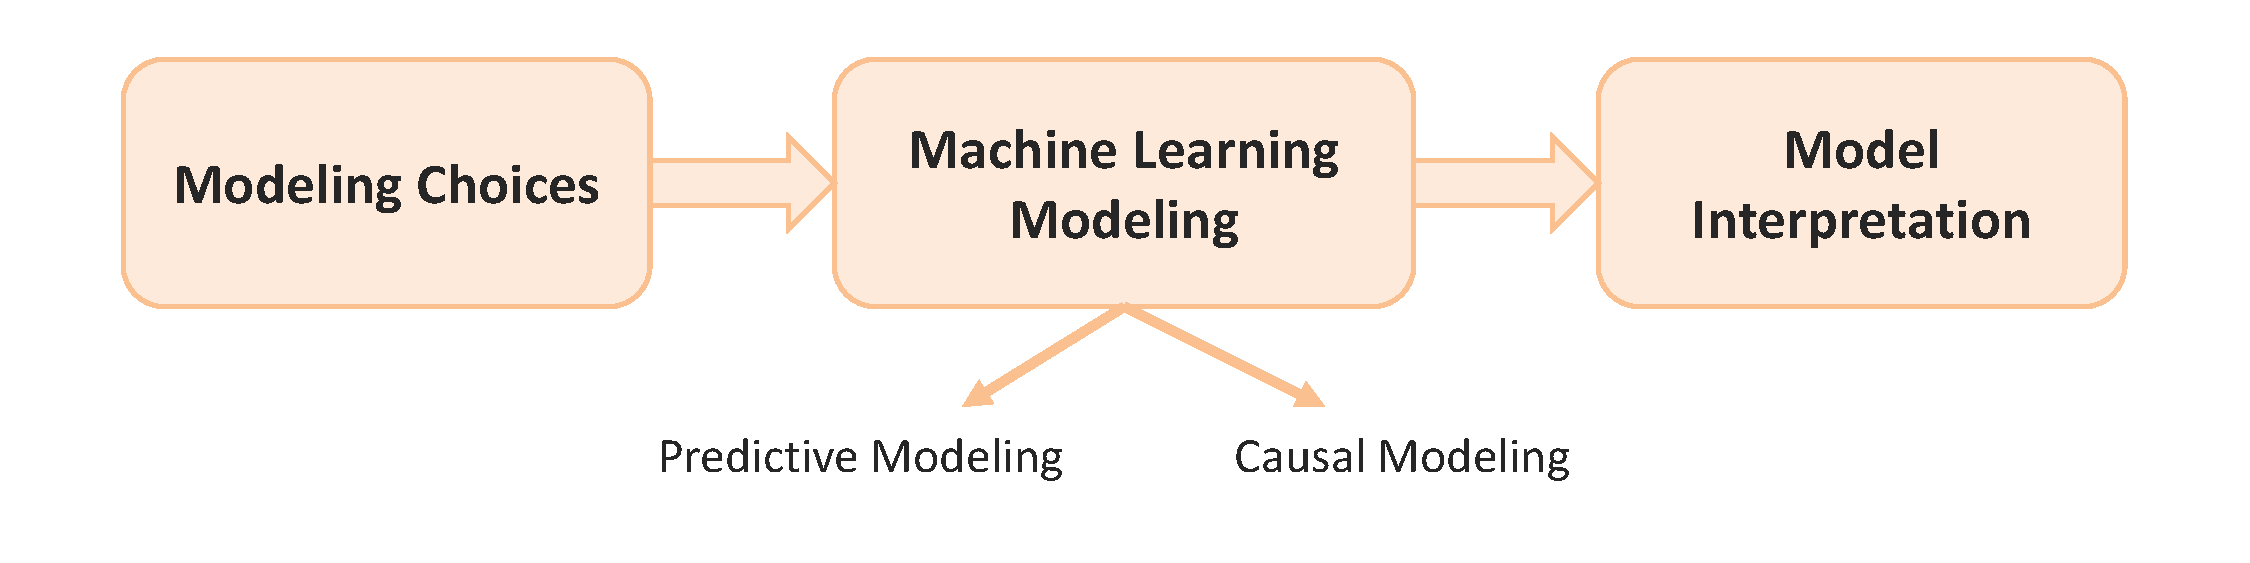
\includegraphics[width=6.5in]{ch1Fig1.pdf}
\caption{Illustration for the typical machine learning modeling pipeline.}
\label{Fig1Ch1}
\end{figure} 

Central to our proposed ML models is the idea of \textit{automation}. In Chapters 4 and 5, we develop methods for making modeling choices in a completely data-driven fashion for both the corss-sectional and longitudinal setups, without the need for manual tuning or expert intervention. Through these automated methods, the ML system is able to craft the model structure by itself so that it best fits the dataset at hand, thereby guarding against na\"ive modeling decisions that may bottleneck the model's predictive accuracy.   \\  
\\ 
\textbf{Stage 2: Machine Learning Modeling}\\
At the core of the modeling pipeline is the actual ML model being used to make predictions. For simple supervised prediction tasks, such as predicting a patient's risk of cardiovascular disease or diabetes based on their age and lifestyle-related variables, one can simply use standard off-the-shelf regression or classification models \cite{weng2017can}. However, many clinical questions cannot be simply reduced to a straightforward prediction problem. As we discuss in detail in Chapter 2, in many cases we would be interested in answering questions such as ``\textit{What is the effect of a given treatment on an individual patient?}'', ``\textit{What is the best treatment option for the patient at hand?}'', or ``\textit{Would this patient have better outcomes had they received a
different medication?}'' For this type of questions, the answer requires inferring the causal effects of interventions, which in turn requires inferring the patient outcomes in counter-factual scenarios that are not observed in the data \cite{morgan2015counterfactuals}. Thus, our core ML models must be able to carry out causal inference tasks and not just predictive inference ones.    

The ML modeling stage should account only for a broad range of clinical questions, but also for different data formats. In the cross-sectional setup, data is simply a static array of variables characterizing the patient state at a given point of time, whereas in the longitudinal setup, data is (irregularly) collected for every patient over time, and each patient may have a different number of observations.  \\ 
\\
\textbf{Stage 3: Model Interpretation}\\
Once the appropriate modeling choices have been made (stage 1), and a model has been trained using the available data (stage 2), we have a functioning ML pipeline in the pragmatic sense --- i.e., we have a model that makes the predictions that we are interested in. However, in almost all clinical setups, this is not enough. An accurate but inscrutable ML model may fail to gain patient and clinician trust. In fact, the conspicuous reluctance of many clinical researchers and epidemiologists to use ML models is often attributed to these models' ``black-box'' nature, which hinders their transparency and interpretability \cite{guidotti2019survey}. 

Because decision support systems based on ML models will be used to inform critical decision-making, clinicians and patients must be able to understand what these models have learned from data and how they makes their predictions. Various regulatory committees have even listed the transparency and intelligibility of prognostic models as a requirement for their deployment \cite{kattan2016american}. The final stage of the ML pipeline thus comprises an interpretation method that enables the users of the ML model to understand its predictions. This stage is inextricable from the preceding stages --- the appropriate kind of model interpretation depends on the ML model being used and format of the data used to train this model. 

\subsection{Outline of the Dissertation}
The rest of this dissertation is organized around the ML pipeline in Figure \ref{Fig1Ch1}. For both the cross-sectional and longitudinal setups, we develop models and algorithms that belong in different stages of the ML pipeline. In what follows, we provide a sneak peek into each of the upcoming chapters, and explain how it relates to the high-level vision in Figure \ref{Fig1Ch1}.  

\label{Sec112}
\subsubsection{Models for Cross-sectional Data} % Technical notation and Figures
Chapters 2, 3 and 4 deal with the 3 stages of the ML pipeline in the cross-sectional setup. In this setup, we examine the relationship between a health outcome $Y$ (e.g., prevalence of a disease, survival outcomes, etc) and patient features $X$ by taking a static ``snapshot of a population'' at a single point of time. (Note that our notion of a ``cross-sectional setup'' corresponds to what is known in the epidemiological literature as \textit{observational studies}, which covers cohort, cross-sectional, and case-control studies.) Chapter 2 starts off with the~core component of the pipeline (stage 2), where we develop a comprehensive framework for ML-based models for causal effect estimation. Chapter 3 proceeds by providing~a~novel symbolic approach for interpreting the predictions of any black-box ML model (stage 3). In Chapter 4, we conclude the ML pipeline for cross-sectional data by developing an algorithm for automating the predictive and causal modeling choices.

\subsubsection{Models for Longitudinal Data}
In Chapter 5, we study the longitudinal setup. In this setup, we are presented sequential data of the form $X_1,.\,.\,.,X_t$ collected for patients who were followed up over an extended period of time. When dealing with longitudinal data, our goal is typically to capture disease trajectories in order to predict patient prognoses in a dynamic fashion and understand the underlying disease mechanisms and dynamics. Unlike in the cross-sectional setup where, in Chapter 5 we do not analyze each stage of the pipeline separately, but rather develop a single comprehensive model for sequential data that executes all stages of the pipeline jointly.     

\subsubsection{Clinical Application}
In Chapter 6, we present a summary of the clinical studies that we conducted based on the ML models developed in earlier chapters. In these studies, we applied our models to cross-sectional data from large-scale cohorts of breast cancer, cardiovascular disease and cystic fibrosis patients, and longitudinal data from the UK cystic fibrosis registry.

\section{Summary of Technical Contributions}
In what follows, we present a brief summary of the technical contributions of each of the upcoming chapters with respect to existing literature.

\label{Sec12}
\subsection*{Chapter 2 Contributions}
In Chapter 2, we consider the problem of using ML to estimate the \textit{causal effect} of a treatment on individual patients on the basis of retrospective, observational data (causal modeling in stage 2 of the pipeline). This problem differs fundamentally from supervised learning since we never observe the treatment effects in the observational data --- we only observe the outcomes of a patient with or without the treatment, but never both. Despite a variety of recently proposed algorithmic solutions to this problem, a principled guideline for building estimators of treatment effects using machine learning algorithms is still lacking. In this chapter, we provide such guidelines by characterizing the fundamental limits of estimating heterogeneous treatment effects, establishing conditions under which these limits can be achieved, and building a practical algorithm for estimating treatment effects based on Gaussian processes. 

\subsection*{Chapter 3 Contributions}
In this Chapter, we tackle stage 3 of the pipeline: understanding the predictions of a general ML model. To this end, we introduce the \textit{symbolic metamodeling} framework --- a general methodology for interpreting predictions by converting ``black-box'' models into ``white-box'' functions that are understandable to human subjects. A symbolic metamodel is a model of a model, i.e., a surrogate model of a trained (machine learning) model expressed through a succinct symbolic expression that comprises familiar mathematical functions and can be subjected to symbolic manipulation. We parameterize metamodels using Meijer $G$-functions --- a class of complex-valued contour integrals that depend on real-valued parameters, and whose solutions reduce to familiar algebraic, analytic and closed-form functions for different parameter settings. This parameterization enables efficient optimization of metamodels via gradient descent, and allows discovering the functional forms learned by a model with minimal a priori assumptions. We show that symbolic metamodeling provides a generalized framework for model interpretation — many common forms of model explanation can be analytically derived from a symbolic metamodel.

\subsection*{Chapter 4 Contributions}
This Chapter addresses stage 1 of the pipeline. We developed an algorithm for automating the design of predictive and causal modeling tailored for clinical prognosis. Our algorithm optimizes ensembles of model configurations efficiently using a novel batched Bayesian optimization (BO) algorithm that learns a low-dimensional decomposition of the models' high-dimensional hyper-parameter space in concurrence with the BO procedure. This is achieved by modeling the models' performances as a black-box function with a Gaussian process prior, and modeling the ``similarities'' between the pipelines' baseline algorithms via a sparse additive kernel with a Dirichlet prior. For causal models, we propose a novel influence function-based approach to estimate their accuracy.

\subsection*{Chapter 5 Contributions}
Chapter 5 focuses on the longitudinal setup, where we develop a sequential model for predicting patient outcomes and understanding disease dynamics. Existing models provide the patient with pragmatic (supervised) predictions of risk, but do not provide the clinician with intelligible (unsupervised) representations of disease pathology. In this Chapter, we develop the \textit{attentive state-space model}, a deep probabilistic model that learns accurate and interpretable structured representations for disease trajectories. Unlike Markovian state-space models, in which state dynamics are memoryless, our model uses an attention mechanism to create ``memoryful'' dynamics, whereby attention weights determine the dependence of future disease states on past medical history. To learn the model parameters from medical records, we develop an inference algorithm that jointly learns a compiled inference network and the model parameters, leveraging the attentive representation to construct a variational approximation of the posterior state distribution. 


\chapter{Estimating Treatment Effects from Observational Data}

For text, let's use the first words out of the ispell dictionary.

\chapter{Symbolic Approaches to Prognostic Model Interpretability}

\chapter{Automated Prognostic Modeling}

\chapter{Deep Probabilistic Modeling of Longitudinal Data}

For text, let's use the first words out of the ispell dictionary.

\chapter{Clinical Application}

\chapter{Conclusions}

\bibliographystyle {unsrt} %{thesis}
\bibliography {thesisrefs}    % bibliography references

\end {document}

